
%% bare_conf.tex
%% V1.3
%% 2007/01/11
%% by Michael Shell
%% See:
%% http://www.michaelshell.org/
%% for current contact information.
%%
%% This is a skeleton file demonstrating the use of IEEEtran.cls
%% (requires IEEEtran.cls version 1.7 or later) with an IEEE conference paper.
%%
%% Support sites:
%% http://www.michaelshell.org/tex/ieeetran/
%% http://www.ctan.org/tex-archive/macros/latex/contrib/IEEEtran/
%% and
%% http://www.ieee.org/

%%*************************************************************************
%% Legal Notice:
%% This code is offered as-is without any warranty either expressed or
%% implied; without even the implied warranty of MERCHANTABILITY or
%% FITNESS FOR A PARTICULAR PURPOSE! 
%% User assumes all risk.
%% In no event shall IEEE or any contributor to this code be liable for
%% any damages or losses, including, but not limited to, incidental,
%% consequential, or any other damages, resulting from the use or misuse
%% of any information contained here.
%%
%% All comments are the opinions of their respective authors and are not
%% necessarily endorsed by the IEEE.
%%
%% This work is distributed under the LaTeX Project Public License (LPPL)
%% ( http://www.latex-project.org/ ) version 1.3, and may be freely used,
%% distributed and modified. A copy of the LPPL, version 1.3, is included
%% in the base LaTeX documentation of all distributions of LaTeX released
%% 2003/12/01 or later.
%% Retain all contribution notices and credits.
%% ** Modified files should be clearly indicated as such, including  **
%% ** renaming them and changing author support contact information. **
%%
%% File list of work: IEEEtran.cls, IEEEtran_HOWTO.pdf, bare_adv.tex,
%%                    bare_conf.tex, bare_jrnl.tex, bare_jrnl_compsoc.tex
%%*************************************************************************

% *** Authors should verify (and, if needed, correct) their LaTeX system  ***
% *** with the testflow diagnostic prior to trusting their LaTeX platform ***
% *** with production work. IEEE's font choices can trigger bugs that do  ***
% *** not appear when using other class files.                            ***
% The testflow support page is at:
% http://www.michaelshell.org/tex/testflow/



% Note that the a4paper option is mainly intended so that authors in
% countries using A4 can easily print to A4 and see how their papers will
% look in print - the typesetting of the document will not typically be
% affected with changes in paper size (but the bottom and side margins will).
% Use the testflow package mentioned above to verify correct handling of
% both paper sizes by the user's LaTeX system.
%
% Also note that the "draftcls" or "draftclsnofoot", not "draft", option
% should be used if it is desired that the figures are to be displayed in
% draft mode.
%
\documentclass[conference, twocolumn]{IEEEtran}
% Add the compsoc option for Computer Society conferences.
%
% If IEEEtran.cls has not been installed into the LaTeX system files,
% manually specify the path to it like:
% \documentclass[conference]{../sty/IEEEtran}





% Some very useful LaTeX packages include:
% (uncomment the ones you want to load)


% *** MISC UTILITY PACKAGES ***
%
%\usepackage{ifpdf}
% Heiko Oberdiek's ifpdf.sty is very useful if you need conditional
% compilation based on whether the output is pdf or dvi.
% usage:
% \ifpdf
%   % pdf code
% \else
%   % dvi code
% \fi
% The latest version of ifpdf.sty can be obtained from:
% http://www.ctan.org/tex-archive/macros/latex/contrib/oberdiek/
% Also, note that IEEEtran.cls V1.7 and later provides a builtin
% \ifCLASSINFOpdf conditional that works the same way.
% When switching from latex to pdflatex and vice-versa, the compiler may
% have to be run twice to clear warning/error messages.






% *** CITATION PACKAGES ***
%
%\usepackage{cite}
% cite.sty was written by Donald Arseneau
% V1.6 and later of IEEEtran pre-defines the format of the cite.sty package
% \cite{} output to follow that of IEEE. Loading the cite package will
% result in citation numbers being automatically sorted and properly
% "compressed/ranged". e.g., [1], [9], [2], [7], [5], [6] without using
% cite.sty will become [1], [2], [5]--[7], [9] using cite.sty. cite.sty's
% \cite will automatically add leading space, if needed. Use cite.sty's
% noadjust option (cite.sty V3.8 and later) if you want to turn this off.
% cite.sty is already installed on most LaTeX systems. Be sure and use
% version 4.0 (2003-05-27) and later if using hyperref.sty. cite.sty does
% not currently provide for hyperlinked citations.
% The latest version can be obtained at:
% http://www.ctan.org/tex-archive/macros/latex/contrib/cite/
% The documentation is contained in the cite.sty file itself.






% *** GRAPHICS RELATED PACKAGES ***
%
\ifCLASSINFOpdf
  % \usepackage[pdftex]{graphicx}
  % declare the path(s) where your graphic files are
  % \graphicspath{{../pdf/}{../jpeg/}}
  % and their extensions so you won't have to specify these with
  % every instance of \includegraphics
  % \DeclareGraphicsExtensions{.pdf,.jpeg,.png}
\else
  % or other class option (dvipsone, dvipdf, if not using dvips). graphicx
  % will default to the driver specified in the system graphics.cfg if no
  % driver is specified.
  % \usepackage[dvips]{graphicx}
  % declare the path(s) where your graphic files are
  % \graphicspath{{../eps/}}
  % and their extensions so you won't have to specify these with
  % every instance of \includegraphics
  % \DeclareGraphicsExtensions{.eps}
\fi
% graphicx was written by David Carlisle and Sebastian Rahtz. It is
% required if you want graphics, photos, etc. graphicx.sty is already
% installed on most LaTeX systems. The latest version and documentation can
% be obtained at: 
% http://www.ctan.org/tex-archive/macros/latex/required/graphics/
% Another good source of documentation is "Using Imported Graphics in
% LaTeX2e" by Keith Reckdahl which can be found as epslatex.ps or
% epslatex.pdf at: http://www.ctan.org/tex-archive/info/
%
% latex, and pdflatex in dvi mode, support graphics in encapsulated
% postscript (.eps) format. pdflatex in pdf mode supports graphics
% in .pdf, .jpeg, .png and .mps (metapost) formats. Users should ensure
% that all non-photo figures use a vector format (.eps, .pdf, .mps) and
% not a bitmapped formats (.jpeg, .png). IEEE frowns on bitmapped formats
% which can result in "jaggedy"/blurry rendering of lines and letters as
% well as large increases in file sizes.
%
% You can find documentation about the pdfTeX application at:
% http://www.tug.org/applications/pdftex





% *** MATH PACKAGES ***
%
%\usepackage[cmex10]{amsmath}
% A popular package from the American Mathematical Society that provides
% many useful and powerful commands for dealing with mathematics. If using
% it, be sure to load this package with the cmex10 option to ensure that
% only type 1 fonts will utilized at all point sizes. Without this option,
% it is possible that some math symbols, particularly those within
% footnotes, will be rendered in bitmap form which will result in a
% document that can not be IEEE Xplore compliant!
%
% Also, note that the amsmath package sets \interdisplaylinepenalty to 10000
% thus preventing page breaks from occurring within multiline equations. Use:
%\interdisplaylinepenalty=2500
% after loading amsmath to restore such page breaks as IEEEtran.cls normally
% does. amsmath.sty is already installed on most LaTeX systems. The latest
% version and documentation can be obtained at:
% http://www.ctan.org/tex-archive/macros/latex/required/amslatex/math/





% *** SPECIALIZED LIST PACKAGES ***
%
%\usepackage{algorithmic}
% algorithmic.sty was written by Peter Williams and Rogerio Brito.
% This package provides an algorithmic environment fo describing algorithms.
% You can use the algorithmic environment in-text or within a figure
% environment to provide for a floating algorithm. Do NOT use the algorithm
% floating environment provided by algorithm.sty (by the same authors) or
% algorithm2e.sty (by Christophe Fiorio) as IEEE does not use dedicated
% algorithm float types and packages that provide these will not provide
% correct IEEE style captions. The latest version and documentation of
% algorithmic.sty can be obtained at:
% http://www.ctan.org/tex-archive/macros/latex/contrib/algorithms/
% There is also a support site at:
% http://algorithms.berlios.de/index.html
% Also of interest may be the (relatively newer and more customizable)
% algorithmicx.sty package by Szasz Janos:
% http://www.ctan.org/tex-archive/macros/latex/contrib/algorithmicx/




% *** ALIGNMENT PACKAGES ***
%
%\usepackage{array}
% Frank Mittelbach's and David Carlisle's array.sty patches and improves
% the standard LaTeX2e array and tabular environments to provide better
% appearance and additional user controls. As the default LaTeX2e table
% generation code is lacking to the point of almost being broken with
% respect to the quality of the end results, all users are strongly
% advised to use an enhanced (at the very least that provided by array.sty)
% set of table tools. array.sty is already installed on most systems. The
% latest version and documentation can be obtained at:
% http://www.ctan.org/tex-archive/macros/latex/required/tools/


%\usepackage{mdwmath}
%\usepackage{mdwtab}
% Also highly recommended is Mark Wooding's extremely powerful MDW tools,
% especially mdwmath.sty and mdwtab.sty which are used to format equations
% and tables, respectively. The MDWtools set is already installed on most
% LaTeX systems. The lastest version and documentation is available at:
% http://www.ctan.org/tex-archive/macros/latex/contrib/mdwtools/


% IEEEtran contains the IEEEeqnarray family of commands that can be used to
% generate multiline equations as well as matrices, tables, etc., of high
% quality.


%\usepackage{eqparbox}
% Also of notable interest is Scott Pakin's eqparbox package for creating
% (automatically sized) equal width boxes - aka "natural width parboxes".
% Available at:
% http://www.ctan.org/tex-archive/macros/latex/contrib/eqparbox/





% *** SUBFIGURE PACKAGES ***
%\usepackage[tight,footnotesize]{subfig}
% subfigure.sty was written by Steven Douglas Cochran. This package makes it
% easy to put subfigures in your figures. e.g., "Figure 1a and 1b". For IEEE
% work, it is a good idea to load it with the tight package option to reduce
% the amount of white space around the subfigures. subfigure.sty is already
% installed on most LaTeX systems. The latest version and documentation can
% be obtained at:
% http://www.ctan.org/tex-archive/obsolete/macros/latex/contrib/subfigure/
% subfigure.sty has been superceeded by subfig.sty.



%\usepackage[caption=false]{caption}
%\usepackage[font=footnotesize]{subfig}
% subfig.sty, also written by Steven Douglas Cochran, is the modern
% replacement for subfigure.sty. However, subfig.sty requires and
% automatically loads Axel Sommerfeldt's caption.sty which will override
% IEEEtran.cls handling of captions and this will result in nonIEEE style
% figure/table captions. To prevent this problem, be sure and preload
% caption.sty with its "caption=false" package option. This is will preserve
% IEEEtran.cls handing of captions. Version 1.3 (2005/06/28) and later 
% (recommended due to many improvements over 1.2) of subfig.sty supports
% the caption=false option directly:
%\usepackage[caption=false,font=footnotesize]{subfig}
%
% The latest version and documentation can be obtained at:
% http://www.ctan.org/tex-archive/macros/latex/contrib/subfig/
% The latest version and documentation of caption.sty can be obtained at:
% http://www.ctan.org/tex-archive/macros/latex/contrib/caption/




% *** FLOAT PACKAGES ***
%
%\usepackage{fixltx2e}
% fixltx2e, the successor to the earlier fix2col.sty, was written by
% Frank Mittelbach and David Carlisle. This package corrects a few problems
% in the LaTeX2e kernel, the most notable of which is that in current
% LaTeX2e releases, the ordering of single and double column floats is not
% guaranteed to be preserved. Thus, an unpatched LaTeX2e can allow a
% single column figure to be placed prior to an earlier double column
% figure. The latest version and documentation can be found at:
% http://www.ctan.org/tex-archive/macros/latex/base/



%\usepackage{stfloats}
% stfloats.sty was written by Sigitas Tolusis. This package gives LaTeX2e
% the ability to do double column floats at the bottom of the page as well
% as the top. (e.g., "\begin{figure*}[!b]" is not normally possible in
% LaTeX2e). It also provides a command:
%\fnbelowfloat
% to enable the placement of footnotes below bottom floats (the standard
% LaTeX2e kernel puts them above bottom floats). This is an invasive package
% which rewrites many portions of the LaTeX2e float routines. It may not work
% with other packages that modify the LaTeX2e float routines. The latest
% version and documentation can be obtained at:
% http://www.ctan.org/tex-archive/macros/latex/contrib/sttools/
% Documentation is contained in the stfloats.sty comments as well as in the
% presfull.pdf file. Do not use the stfloats baselinefloat ability as IEEE
% does not allow \baselineskip to stretch. Authors submitting work to the
% IEEE should note that IEEE rarely uses double column equations and
% that authors should try to avoid such use. Do not be tempted to use the
% cuted.sty or midfloat.sty packages (also by Sigitas Tolusis) as IEEE does
% not format its papers in such ways.





% *** PDF, URL AND HYPERLINK PACKAGES ***
%
%\usepackage{url}
% url.sty was written by Donald Arseneau. It provides better support for
% handling and breaking URLs. url.sty is already installed on most LaTeX
% systems. The latest version can be obtained at:
% http://www.ctan.org/tex-archive/macros/latex/contrib/misc/
% Read the url.sty source comments for usage information. Basically,
% \url{my_url_here}.





% *** Do not adjust lengths that control margins, column widths, etc. ***
% *** Do not use packages that alter fonts (such as pslatex).         ***
% There should be no need to do such things with IEEEtran.cls V1.6 and later.
% (Unless specifically asked to do so by the journal or conference you plan
% to submit to, of course. )


% correct bad hyphenation here
\hyphenation{op-tical net-works semi-conduc-tor}

% Additions for multi-robot motion planning
\usepackage{graphicx}        % standard LaTeX graphics tool
                             % when including figure file

%% Added from Lyx generated code
\usepackage{nomencl} % allows for nomenclature entries
\usepackage{subcaption} % allows for subfigures
\usepackage{amsthm} % allow for newtheorem
\newtheorem*{defi}{Definition} % allow for our custom definitions
\usepackage{float} % allow for algorithms
    \newfloat{algorithm}{tbp}{loa}
    \providecommand{\algorithmname}{Algorithm}
    \floatname{algorithm}{\protect\algorithmname}
    \usepackage{listings}
	
%\usepackage[hmargin=0.8in, top=1in, bottom=0.8in]{geometry}
\usepackage[hmargin=0.5in, top=0.5in, bottom=0.5in]{geometry}
\usepackage{flushend}
\usepackage{siunitx}
\usepackage{color}

% custom commands
\newcommand{\noun}[1]{\textsc{#1}}
\newcommand{\tn}{\textnormal}
\newcommand{\tb}{\textbf}
\newcommand{\ti}{\emph}

\newcommand{\rs}{r^*}
\newcommand{\rlbs}{\underline{r}^*}
\newcommand{\rhbs}{\overline{r}^*}
\newcommand{\courier}{\fontfamily{pcr}\selectfont}

\newcommand{\degree}{^{\circ}}

\begin{document}
%
% paper title
% can use linebreaks \\ within to get better formatting as desired
%\title{Bare Demo of IEEEtran.cls for Conferences}


% author names and affiliations
% use a multiple column layout for up to three different
% affiliations
%\author{\IEEEauthorblockN{Michael Shell}
%\IEEEauthorblockA{School of Electrical and\\Computer Engineering\\
%Georgia Institute of Technology\\
%Atlanta, Georgia 30332--0250\\
%Email: http://www.michaelshell.org/contact.html}
%\and
%\IEEEauthorblockN{Homer Simpson}
%\IEEEauthorblockA{Twentieth Century Fox\\
%Springfield, USA\\
%Email: homer@thesimpsons.com}
%\and
%\IEEEauthorblockN{James Kirk\\ and Montgomery Scott}
%\IEEEauthorblockA{Starfleet Academy\\
%San Francisco, California 96678-2391\\
%Telephone: (800) 555--1212\\
%Fax: (888) 555--1212}}

\title{SHaZam the Magic Lamp:\\IR-Based Gaze Tracking and Light Direction}
%\author{Adam Wiktor, Dexter Scobee, Sean Messenger and Christopher Clark}
%\institute{Adam Wiktor \at Princeton University, Princeton, NJ 08544, \email{awiktor@alumni.princeton.edu} 
%\and Dexter Scobee \at Princeton University, Princeton, NJ 08544, \email{dscobee@alumni.princeton.edu}
%\and Christopher Clark \at Engineering Dept., Harvey Mudd College, Claremont, CA 91711, \email{clark@hmc.edu}}


% conference papers do not typically use \thanks and this command
% is locked out in conference mode. If really needed, such as for
% the acknowledgment of grants, issue a \IEEEoverridecommandlockouts
% after \documentclass

% for over three affiliations, or if they all won't fit within the width
% of the page, use this alternative format:
% 
%\author{\IEEEauthorblockN{Michael Shell\IEEEauthorrefmark{1},
%Homer Simpson\IEEEauthorrefmark{2},
%James Kirk\IEEEauthorrefmark{3}, 
%Montgomery Scott\IEEEauthorrefmark{3} and
%Eldon Tyrell\IEEEauthorrefmark{4}}
%\IEEEauthorblockA{\IEEEauthorrefmark{1}School of Electrical and Computer Engineering\\
%Georgia Institute of Technology,
%Atlanta, Georgia 30332--0250\\ Email: see http://www.michaelshell.org/contact.html}
%\IEEEauthorblockA{\IEEEauthorrefmark{2}Twentieth Century Fox, Springfield, USA\\
%Email: homer@thesimpsons.com}
%\IEEEauthorblockA{\IEEEauthorrefmark{3}Starfleet Academy, San Francisco, California 96678-2391\\
%Telephone: (800) 555--1212, Fax: (888) 555--1212}
%\IEEEauthorblockA{\IEEEauthorrefmark{4}Tyrell Inc., 123 Replicant Street, Los Angeles, California 90210--4321}}

%\author{\IEEEauthorblockN{Chaim Halbert\IEEEauthorrefmark{1},
%Dexter Scobee\IEEEauthorrefmark{1}, and
%Edward Zhao\IEEEauthorrefmark{1}}
%%\IEEEauthorblockA{\IEEEauthorrefmark{1}University of California, Berkeley\\Department of Electrical Engineering and Computer Sciences}}
%%\IEEEauthorblockA{\IEEEauthorrefmark{3}Starfleet Academy, San Francisco, California 96678-2391\\
%%Telephone: (800) 555--1212, Fax: (888) 555--1212}
%%\IEEEauthorblockA{\IEEEauthorrefmark{4}Tyrell Inc., 123 Replicant Street, Los Angeles, California 90210--4321}}

\author{\IEEEauthorblockN{Chaim Halbert,
Dexter Scobee, and
Edward Zhao}
\IEEEauthorblockA{EE149A/EE249A Project Final Report}}
%\IEEEauthorblockA{\IEEEauthorrefmark{3}Starfleet Academy, San Francisco, California 96678-2391\\
%Telephone: (800) 555--1212, Fax: (888) 555--1212}
%\IEEEauthorblockA{\IEEEauthorrefmark{4}Tyrell Inc., 123 Replicant Street, Los Angeles, California 90210--4321}}


% use for special paper notices
%\IEEEspecialpapernotice{(Invited Paper)}




% make the title area
\maketitle


%\begin{abstract}
%%\boldmath
%%The abstract goes here.
%\end{abstract}

% IEEEtran.cls defaults to using nonbold math in the Abstract.
% This preserves the distinction between vectors and scalars. However,
% if the conference you are submitting to favors bold math in the abstract,
% then you can use LaTeX's standard command \boldmath at the very start
% of the abstract to achieve this. Many IEEE journals/conferences frown on
% math in the abstract anyway.

% no keywords




% For peer review papers, you can put extra information on the cover
% page as needed:
% \ifCLASSOPTIONpeerreview
% \begin{center} \bfseries EDICS Category: 3-BBND \end{center}
% \fi
%
% For peerreview papers, this IEEEtran command inserts a page break and
% creates the second title. It will be ignored for other modes.
\IEEEpeerreviewmaketitle



\section{Project Vision}
% no \IEEEPARstart
%This demo file is intended to serve as a ``starter file''
%for IEEE conference papers produced under \LaTeX\ using
%IEEEtran.cls version 1.7 and later.
%% You must have at least 2 lines in the paragraph with the drop letter
%% (should never be an issue)
%I wish you the best of success.

The goal of this project was to design a lamp that will redirect its light to follow a user's gaze. The magic lamp will consist of a flashlight attached to a two-axis motor assembly, to be directed by an embedded microcontroller. Additionally, the lamp will utilize a Wiimote to track IR LEDs affixed to a specially designed hat. The Wiimote will communicate relative positioning data to the microcontroller via Bluetooth, which will in turn direct the motors to aim the flashlight. The controller will behave according to a state-machine that describes both automatic and manual modes of behvior. Figure \ref{fig:conops} shows the logical connections between system components and how they are intended to interact, and Figure \ref{fig:state_machines} depicts the governing state machines.

\begin{figure}[!t]
\begin{center}
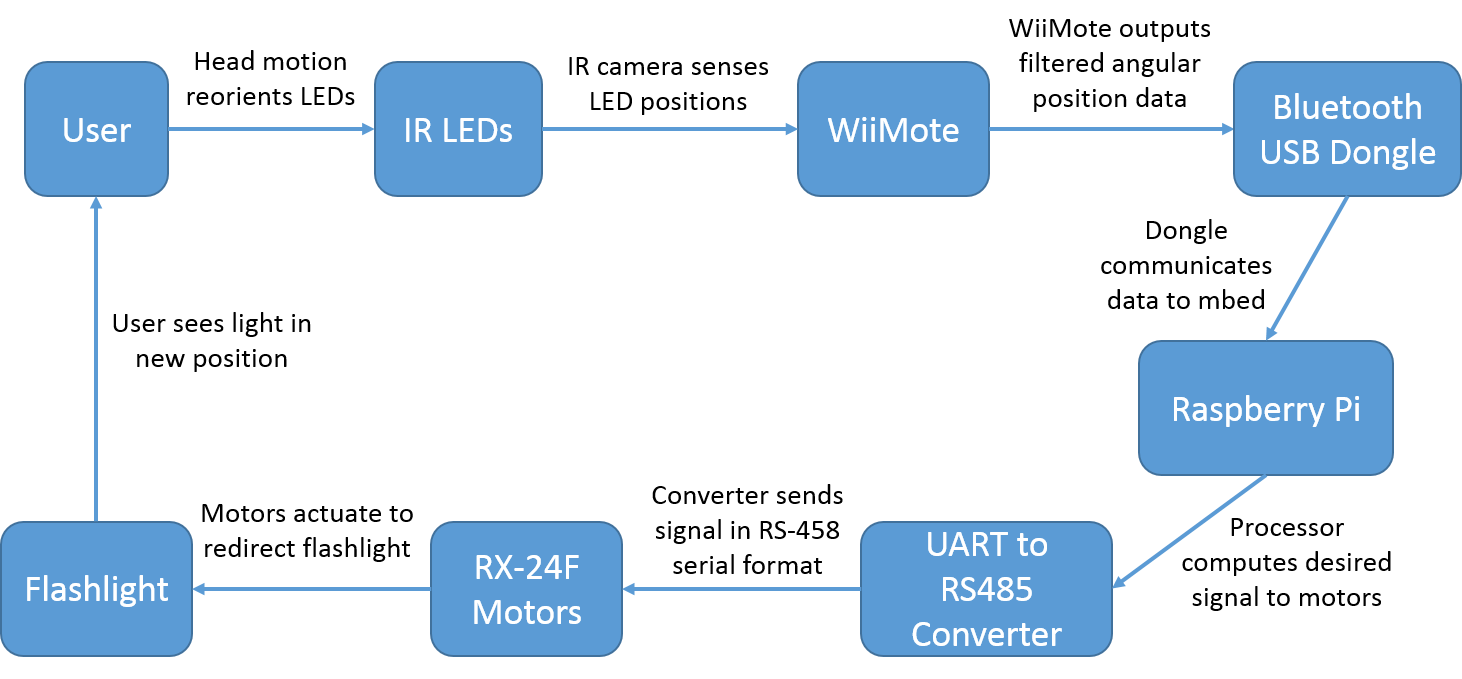
\includegraphics[width=\linewidth]{../images/conops_update}
\end{center}

\caption{SHaZam ConOps. This diagram represents the interconnections between components for the SHaZam system}
\label{fig:conops}
\end{figure}

\section{Hardware}
\label{sec:hardware}
The hardware consists of a gimbal-mounted flashlight connected to a system controller, in turn connected wirelessly to a Wiimote, which tracks sensor bars mounted on the user's hat.

The gimbal is a pair of Dynamixel \mbox{RX-24F} smart servos, which are daisy-chained and connected to the system controller via \mbox{RS-485} serial link. To convert the \mbox{RS-485} to 3.3V serial UART, we used an SP3485 breakout board.

The system controller is a Raspberry Pi running Raspbian Linux in ``headless'' configuration, without a monitor, keyboard or mouse. These can be added for development and debugging, or an ethernet connection can be used to log in remotely via SSH.

The system controller links to the Wiimote via a USB Bluetooth dongle. (Somehow, we had issues with newer Wiimotes that included MotionPlus, so we used an older Wiimote without it.) The WiiBrew web site \footnote{http://wiibrew.org/wiki/Wiimote} was a valuable resource in understanding the Wiimote hardware and in interfacing the Wiimote with the system controller.

The hat has two Wii ``sensor bars'' mounted to it. These bars are not sensors at all, but actually contain a simple collection of IR LEDs at either end of each. The specially-designed camera in the Wiimote picks up and tracks these four points of invisible light. For more information about the sensor bars' asymmetrical configuration, see section \ref{sec:algorithms}.

\subsection*{Design changes}
Although the overall structure and linkages of our system diagram have not changed since the beginning of our project, virtually every block was modified by the end of development.

\subsubsection{Gimbal}
Our original design called for traditional servo motors to drive the gimbal's motion, but we decided to change to advanced, serially-controlled servos. These Dynamixel \mbox{RX-24F} motors (see Figure \ref{fig:hw_mk0}) provided several advantages, the primary one being ease of control.

Unlike traditional servo motors which are commanded to set their position using PWM, our smart servos could be commanded via \mbox{RS-485} serial link. This provides more timing flexibility in our control logic, since this makes PWM interrupt routines unnecessary. The smart servos also allowed us to set the speed of the movements over the serial link, offloading logic from our main control loop to the motors.

Also, the new servos were daisy-chainable, an impossibility with PWM. This allowed us to use a single serial output, as opposed to multiple, independent PWM outputs, each with their own interrupt routines. This resulted in a subtantial time savings in development, and greater reliability.

A disadvantage was that \mbox{RS-485} is quite different from serial UART, in that it uses \mbox{200 mV} differential signaling over two wires and is half-duplex, whereas our TTL UART operates at 3.3V and is full-duplex. We used a breakout board for the SP3485, which accomplishes both level conversion and protocol translation, with the aid of an RTS signal from our system controller's GPIO.

\subsubsection{Bluetooth}
Originally, we planned to use a BlueSMiRF Gold to connect to the Wiimote. However, the Gold only connects via serial data endpoints, while the Wiimote requires an HID interface. So, the BlueSMiRF Gold did not work.

To resolve this problem, we purchased a BlueSMiRF HID, which has the same hardware as the BlueSMiRF Gold, but has different factory-flashed firmware for HID capabilities. This also did not work, because the BlueSMiRF HID was designed to operate as an HID slave device, such as a mouse, keyboard or joystick; it could not operate as an HID host, to control such HID devices.

In the end, we used a USB-Bluetooth dongle.

\subsubsection{System controller}
Although we originally intended to use the ARM mbed \mbox{FRDM-KL25Z} Freedom board, we decided to change platforms to the Raspberry Pi model B.

We did not use the Pi initially because the lab already provided each of our group members with a free, personal ARM mbed processor. This allowed us to work independently, parallelizing development. In comparison, the Pi cost \$35. Also, PWM control requires Linux kernel programming on the Pi, or a separate daughterboard with its own microprocessor, such as the Arduino-compatible Pi Alamode (another \$35). We deemed this too complex and expensive.

However, circumstances changed during development. By switching to the serial servos, we eliminated the need for kernel programming or a daughterboard. Just like with the ARM mbed, we could now control all the hardware with a single system controller. Also, when we exchanged the BlueSMiRF for the Bluetooth dongle, the easily-installed support for the dongle in Linux gave the Pi a clear advantage over the ARM mbed, which in contrast required compiling and integrating C++ code. The Pi was simpler.

The Pi also offered new capabilities not available on ARM mbed. With the Pi, we could change languages from C++ to Python, and we could develop and test directly on the Pi itself. This eliminated the need for compilation and flashing every time we made a change. It also gave us an interactive Python shell to test out snippets of code prior to integration.

Next was the ethernet connection on the Pi. Connected to a LAN, multiple members could work simultaneously on the Pi via SSH. Also, with an internet connection, we could use package managers to quickly install and test pre-built third-party modules for new Linux and Python functionality. The internet also gave us tighter integration with GitHub for version tracking and merging our code modifications. The confidence that we could quickly revert our changes allowed rapid progress even as the deadline approached.

\begin{figure}[!t]
\begin{center}
%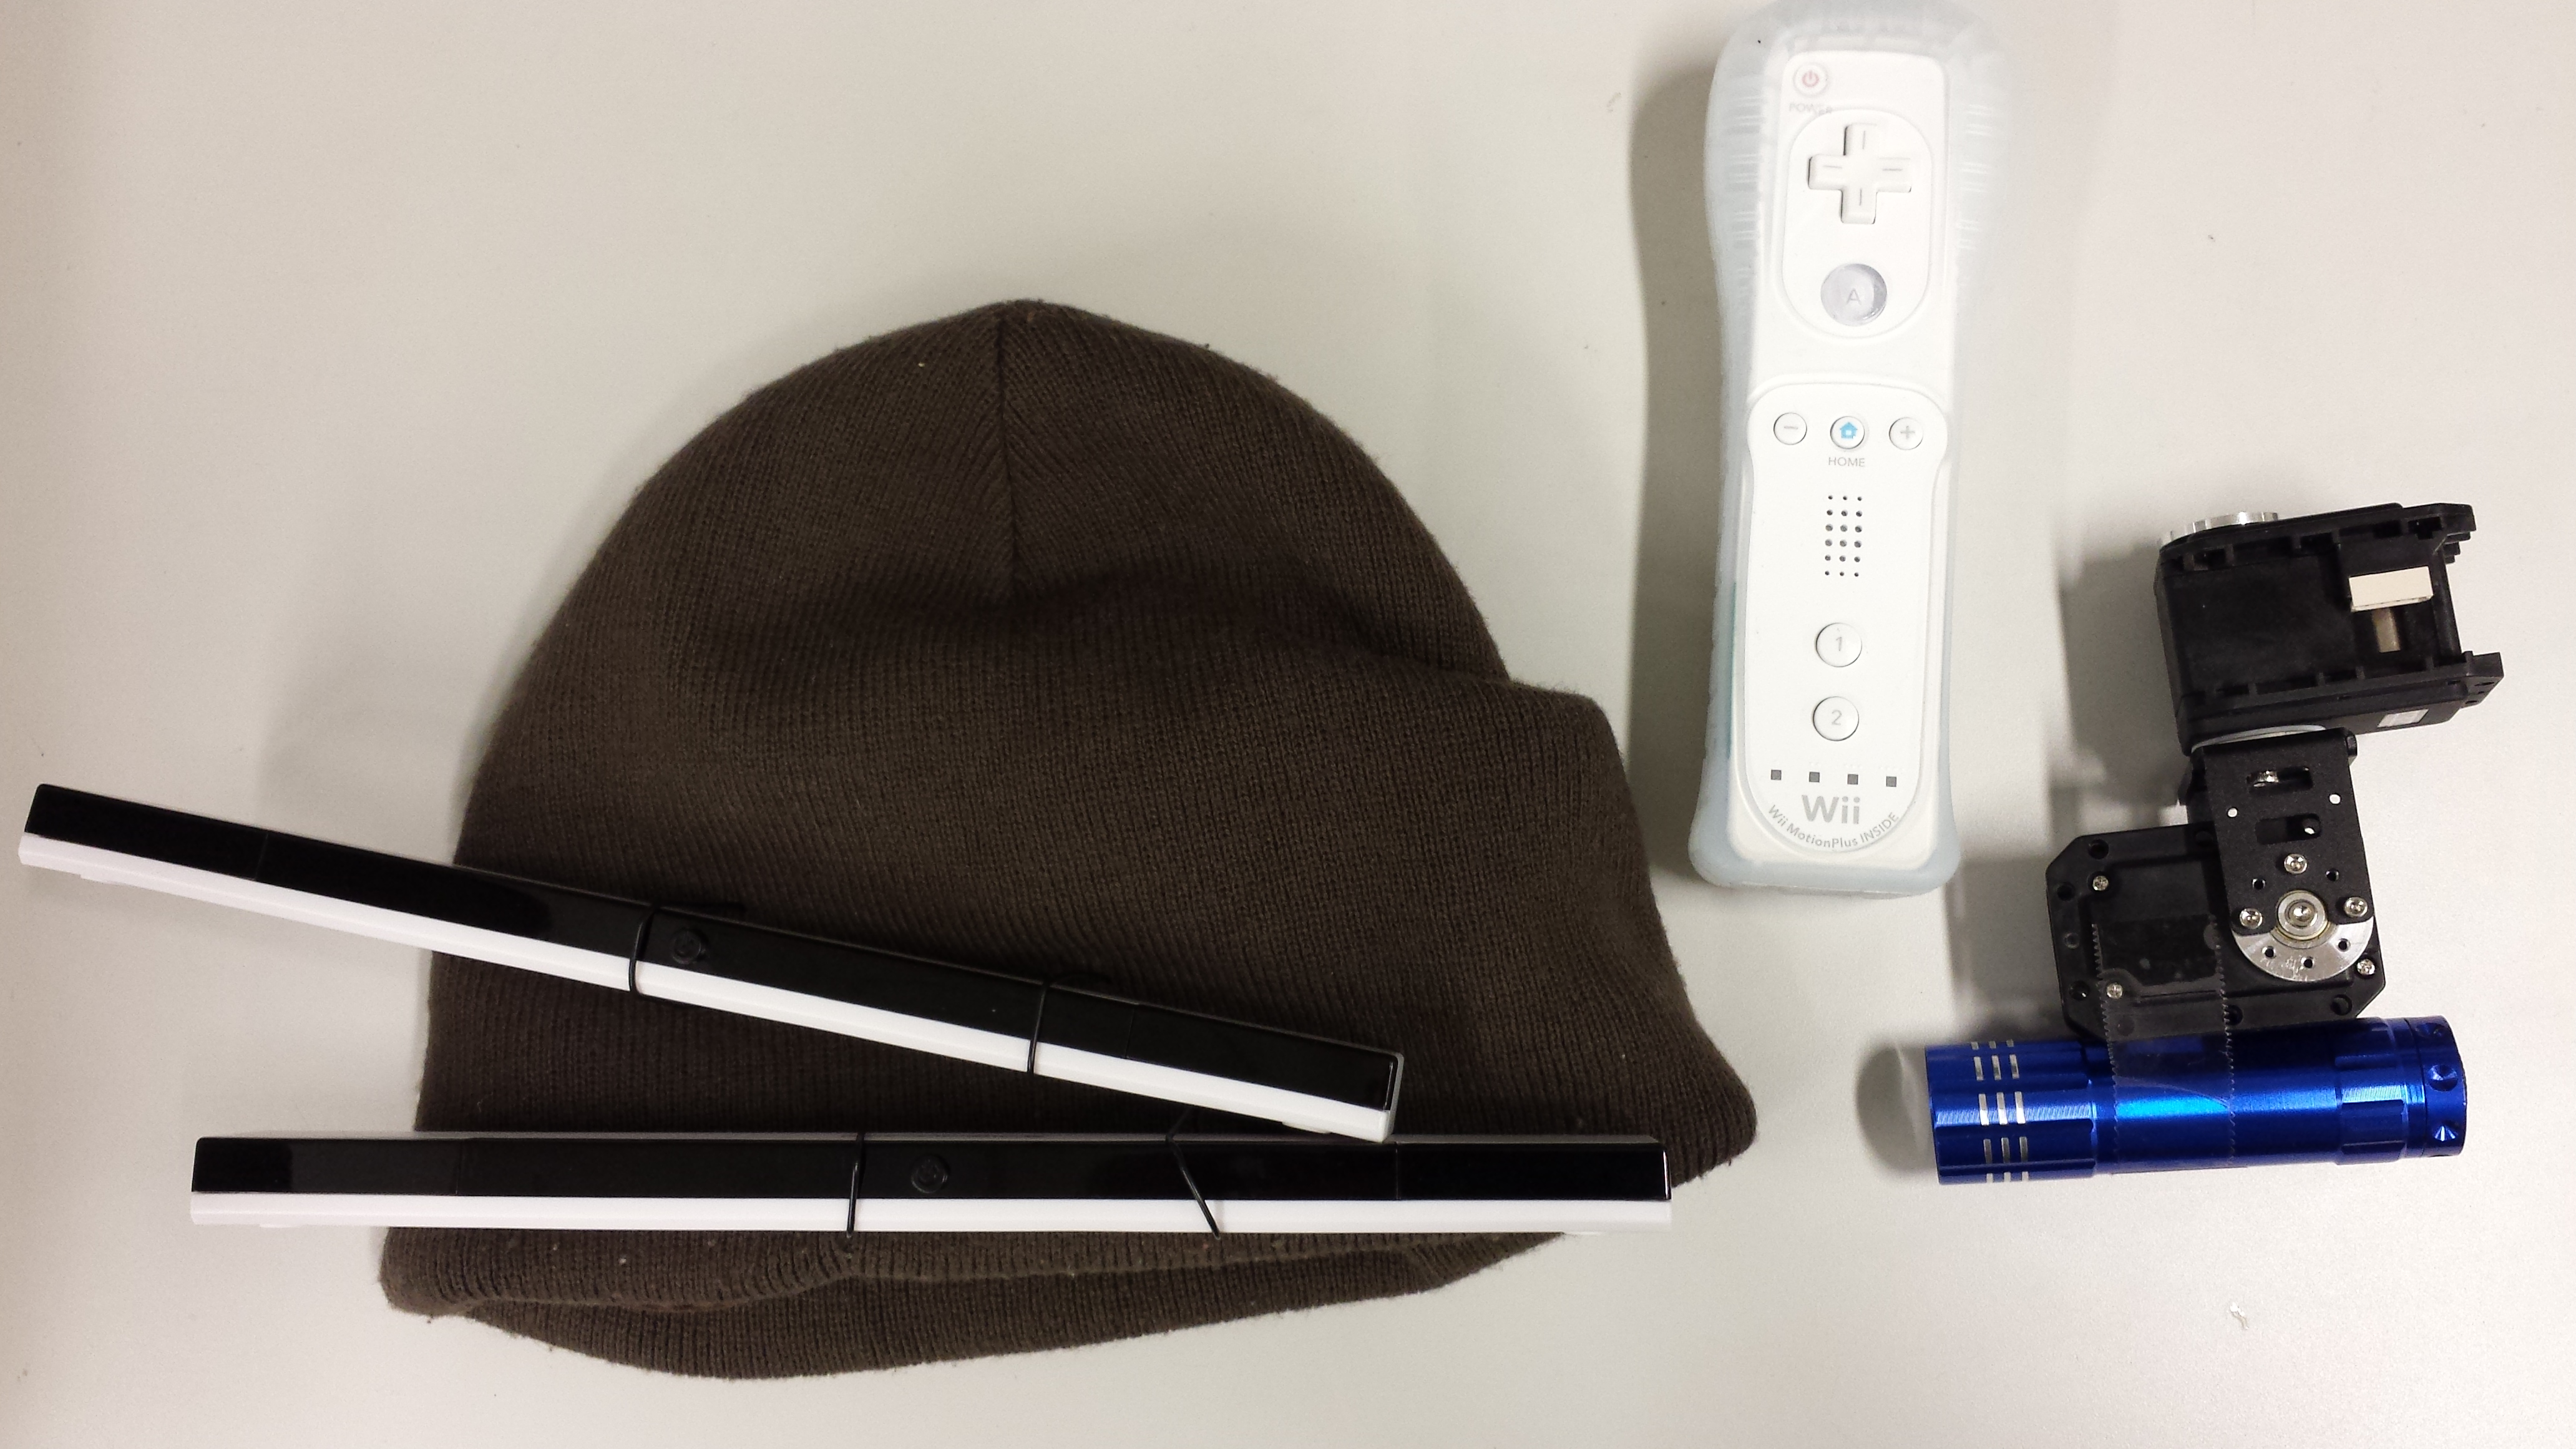
\includegraphics[height=5.2cm]{../images/hw_mk0}
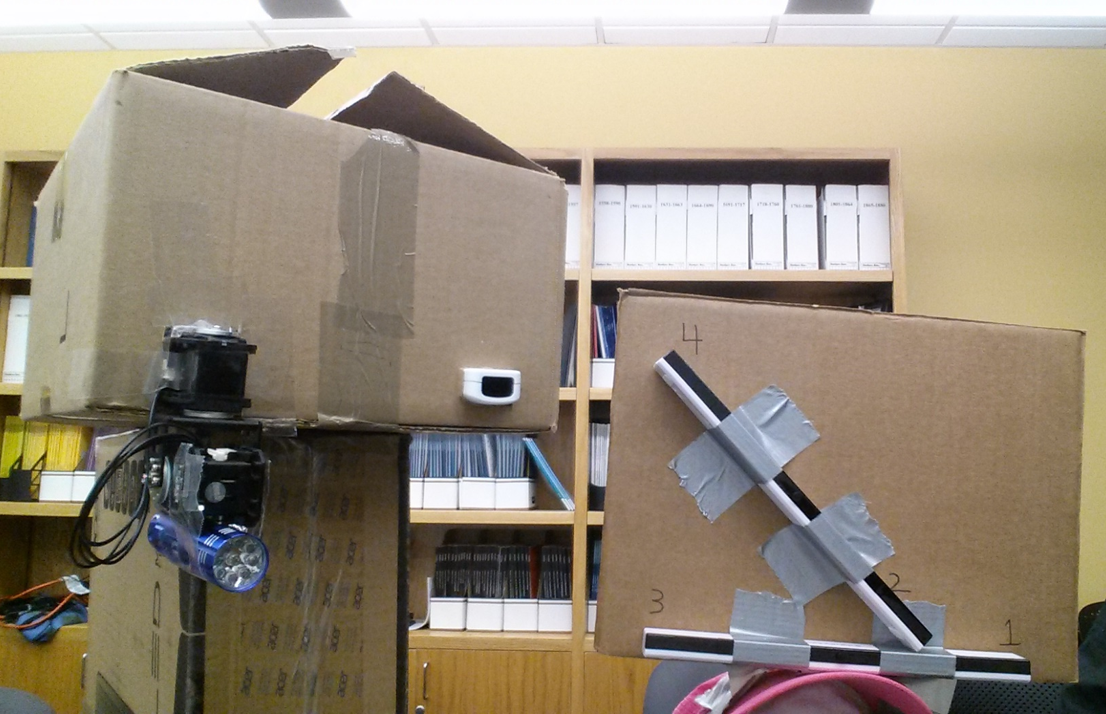
\includegraphics[width=\linewidth]{../images/shazam_outer2}
\end{center}

\caption{SHaZam External Hardware. On the left, the main console with a protruding Wiimote camera and a Dynamixel 2-axis motor assembly with an attached flashlight. On the right, the head-mounted IR LED assembly for user wear.}
\label{fig:hw_mk0}
\end{figure}

\begin{figure}[!t]
\begin{center}
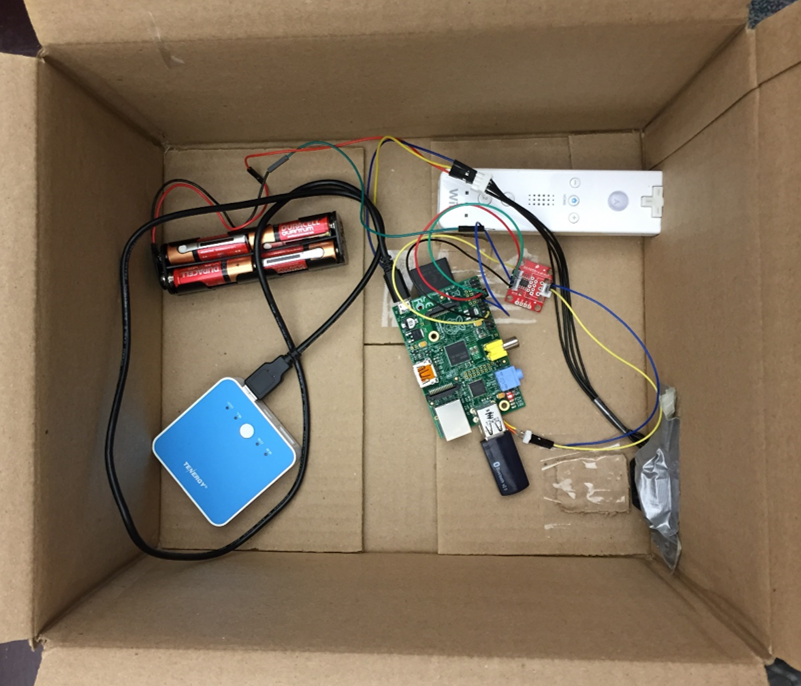
\includegraphics[width=0.8\linewidth]{../images/shazam_inner}
\end{center}

\caption{SHaZam Internal Hardware. Clockwise, from top: Wiimote, Sparkfun RS485 breakout board, Raspberry Pi with attached Bluetooth dongle, USB power module for the Raspberry Pi, Battery assembly (8 AA) for powering motors.}
\label{fig:hw_inner}
\end{figure}

\section{Software}
On the Raspberry Pi platform, we opted to utilize Python as our language of choice. The reason for that is twofold; the first is that there is an extensive library called CWiiD\footnote{CWiiD was developed by Donnie Smith of Georgia Tech - https://github.com/abstrakraft/cwiid}, which provided a robust API to interface with the Wiimote. The second reason was that, once we had decided to use the Pi and its full Linux capability (see section \ref{sec:hardware}), we wanted to use a language with which we had more experience coding and debugging, cutting down development time by significant margins. 

In the actual code, the main logic resides in statechart.py. The state machine logic, connection to the Wiimote via CWiiD, and sample logic all reside in this file. Essentially, we run a while loop, sampling every 0.2 seconds for IR position data. Based on this data, we used the modeling algorithms (described in section \ref{sec:algorithms}) to find the appropriate pitch and yaw angle, then move the motors to that angle. We had to introduce a small amount of asynchronous behavior in order to receive the latest input data from the Wiimote. This is because periodic polling with get\_mesg() yields only the oldest undelivered data, which is not sufficient for our purposes. In our solution, CWiiD is set to continuously receive IR camera and button status data. Every time CWiiD receives a new message, it invokes a callback which updates variables with our input data and updates our FSM state. For instance, if we detect button A being pressed, we immediately update our state to go into Manual Mode. This was difficult with purely synchronous updating, since the output of get\_mesg() was almost always out-of-date.

We import a file in statechart called motor\_control, which is responsible for changing the motor positions via serial link. Once the desired pitch and yaw commands are calculated in statechart.py, and deemed to be within the designed range of motion, they are passed into motor\_control.py. Motor\_control.py then takes this data, and calculates the difference between the desired pitch and yaw and its current pitch and yaw, and finds the necessary speed needed to reconcile that difference. Once this is calculated, motor\_control.py constructs a serial packet and sends it via the \mbox{RS-485} converter to the motors. The motor microcontrollers take over from there, driving the servos to track the user.

\section{Modeling and Algorithms}
\label{sec:algorithms}
We developed a finite state machine that models the behavior we want for our project, as well as mathematical models detailing our tracking algorithm.
 
 \subsection*{FSM System Model}
 The SHaZam system can be modeled as a hierarchical composition of state machines. At the highest level (shown in Figure \ref{fig:high_state}) the system starts by looking to pair via Bluetooth with a Wiimote (state BLUETOOTH\_PAIRING), and continues doing so until it successfully pairs. This is the state first entered when the sytem is turned on.
 
 Once paired, the system will transition to AUTO mode, which enables tracking of the user position. Within AUTO, there are two identical yet separate state machines for controlling the motors pitch and yaw. Figure \ref{fig:auto_state} shows the FSM model for these machines. The system begins in the STAY state for both angular axes. For a given axis, if the motor are commanded to change its angle by a value which is within our accepted bounds (described in the figure as the range between minThresh and maxThresh) then the system transitions to TRACK and the lamp will be reoriented to point at the appropriate location. If the angular command falls outside of this range, that command is ignored and the system remains in STAY (in this case, the calculated command is never actually sent to the motors). Once in TRACK, if the change in angle is below minThresh (the desired lamp position has settled) or the change is above maxThresh (likely due to an errant measurement), then the system returns to STAY and holds its position.
 
If the user pushes the ``A'' button on the Wiimote, the system will transition into MANUAL (the manual mode is represented in Figure \ref{fig:manual_state}). This sub-state machine follows a similar model to AUTO in that it also transitions back and forth between a stationary state (NotButtonPress) and a moving state (ButtonPressed). As the state names suggest, the transition is triggered by the pressing or releasing of buttons on the Wiimote. In ButtonPressed, the change in motor position is determined by which button is being pressed, and at every time increment (recall that our sample time is 0.2 seconds) the appropriate change occurs. Unlike AUTO, MANUAL has a third state, labeled Rumble. When a button is pressed that would have commanded the system to move beyond its designed range of motion, the system transitions to Rumble in lieu of ButtonPressed. In Rumble, the system remains stationary and vibrates to alert the user that they have reached the bounds of motion.

Finally, if the user presses ``A'' and ``B'' simultaneously on the Wiimote, the system will transition from MANUAL back to AUTO, allowing the user to change between these two modes of operation at their discretion.

\subsection*{User State Estimation}
We have also derived a mathematical model that will allow us to reconstuct the state of the LED configuration (which reveals where the user is looking) by obtaining angular position measurements from the Wiimote.\footnote{This model is an expansion of work done by Johnny Chung Lee (Google, formerly CMU). See http://johnnylee.net/projects/wii/} The data provided are x- and y-angle measurements, corresponding to the estimated angular position of the LEDs in two orthogonal planes. Figure \ref{fig:geometry} shows the geometry of reconstructing the state in one of these measurement planes. Note that the state of the LEDs in a plane has three degrees of freedom (shown in Figure \ref{fig:geometry} as $x_{3}$, $y_{3}$, and $\psi_{user}$), so three angular measurements are needed to unambiguously reconstruct the state. Once the state in the first plane is known, however, the range data ($x_3$) is known for the second plane as well, so only two angular measurements are needed to reconstruct the state relative to the second plane. 

\subsection*{Command Generation}
Given the user's head position (x,y,z) and orientation (pitch $\theta$ and yaw $\psi$), we could then use a second algorithm to calculate where the user's line of sight would intersect with the surface of the table upon which the SHaZam system was placed. Once that location was known, it was then possible to calculate the required pitch and yaw of the lamp to shine a light such that it would also intersect the table at that same location. This process of calculating the intersection location based on user angles and then the required lamp angles based on the intersection location was accomplished using standard trigonometric and inverse trigonometric functions.

\subsection*{Verification and Testing}
In order to verify the accuracy of these solutions, we created a simple model of the system in MATLAB that allowed us to specify user state data (angular and positional state), determine where the LEDs would appear relative to the Wiimote camera, and use that data to drive our state estimation and command generation algorithms. After successfully recreating our input state data based on expected measurements, the simulation indicated that we had derived an exact solution to the problem. However, upon running our algorithm using actual data collected by the Wiimote, we soon discovered that even in a static configuration (minimal motion of the Wiimote and the LEDs) the estimated angular state of the user exhibited large variations that would give erratic data to the command generation algorithm, and would have resulted in extraneous lamp motion. We confirmed this numerical instability in our MATLAB simulation, noticing that even a $1\degree$ error in a single measurement could result in nearly $50\degree$ of error in the user orientation estimate.

\subsection*{Managing Noisy Data}
While the estimated angular state of the user was determined to be unusable (varying by tens of degrees), the estimated user position was notably more stable (varying on the order of one or two centimeters). It was therefore decided to re-scope our design to focus on directing the lamp at the user themselves. This change was accomplished without significant variation to our existing state estimation algorithm (we were already estimating positional data) or our command generation algorithm (we substituted the user's head position for the position of their gaze upon the table). To further ensure that the motors would not be commanded to move erratically, we tuned the angular change thresholds used in our state machine to allow the motors to respond to meaningful small changes while ignoring extraneous large changes which may be caused by measurement anomalies. Future implementations may consider applying various filtering schemes to smooth out state estimates and acheive gaze tracking capability.

\subsection*{Manual Mode}
Operating the system in manual mode proved to be more straightforward as it did not rely on camera measurements taken by the Wiimote. In this mode, directional input from the Wiimote D-pad was used to increment or decrement the pitch or yaw of the motor assembly. If the user tried to command either a pitch or yaw angle that was outside of the designed range of motion, the command would not be executed and the Wiimote would rumble to alert the user to the fact that they had reached the system bounds.

\begin{figure}
\begin{center}
    \begin{subfigure}[b]{0.7\linewidth}
    \begin{center}
    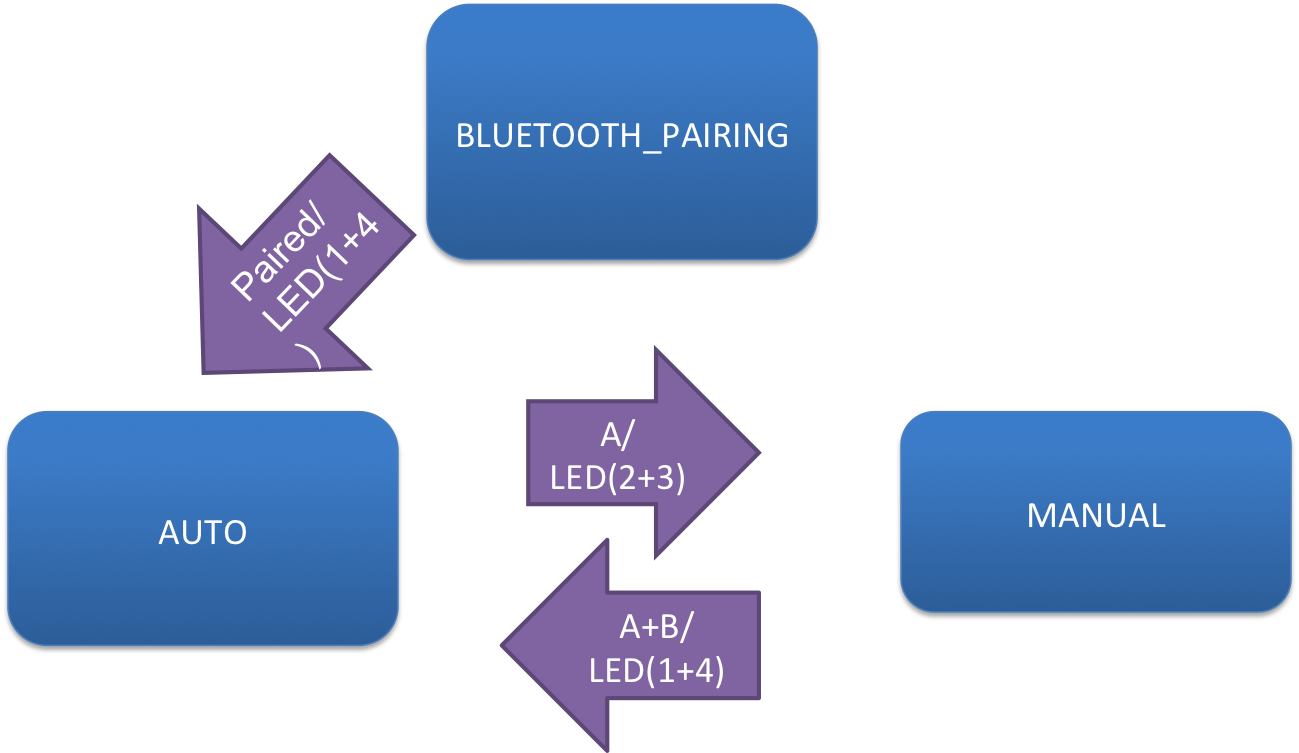
\includegraphics[width=1\linewidth]{../images/high_state}
    \caption{Top-level state machine model}
    \label{fig:high_state}
    \end{center}
    \end{subfigure}
    
    \vspace{0.05\linewidth}
    
    \begin{subfigure}[b]{0.7\linewidth}
    \begin{center}
    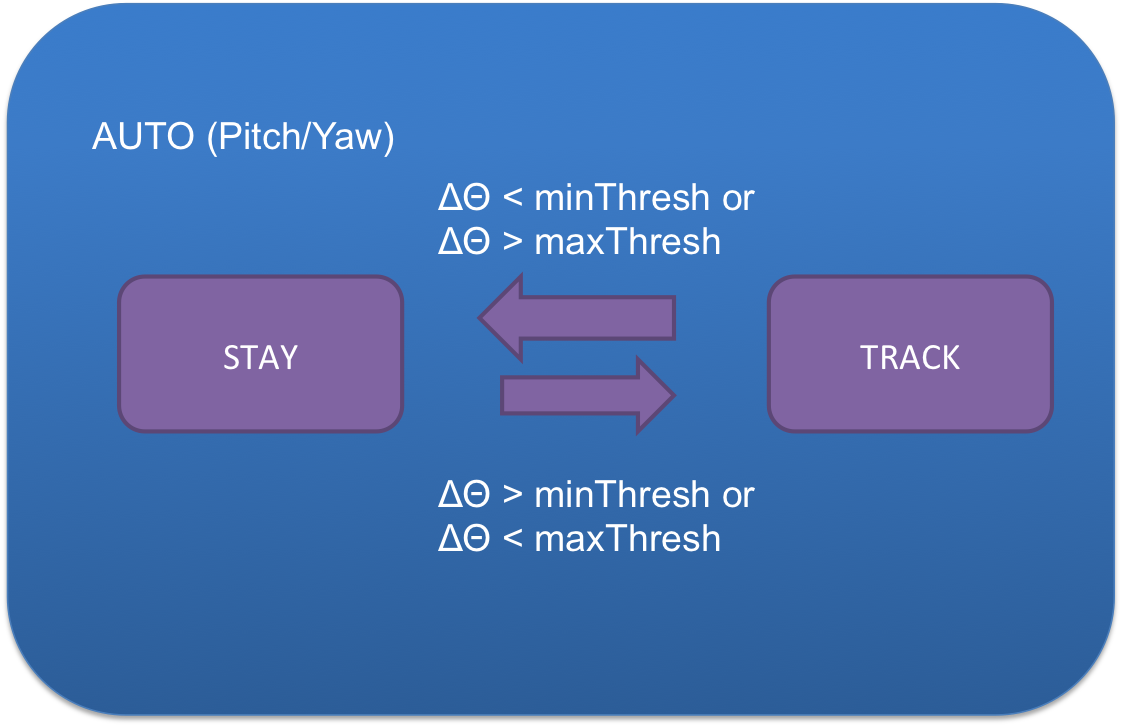
\includegraphics[width=1\linewidth]{../images/auto}
    \caption{Automated mode state machine model}
    \label{fig:auto_state}
    \end{center}
    \end{subfigure}
    
    \vspace{0.05\linewidth}
    
    \begin{subfigure}[b]{0.7\linewidth}
    \begin{center}
    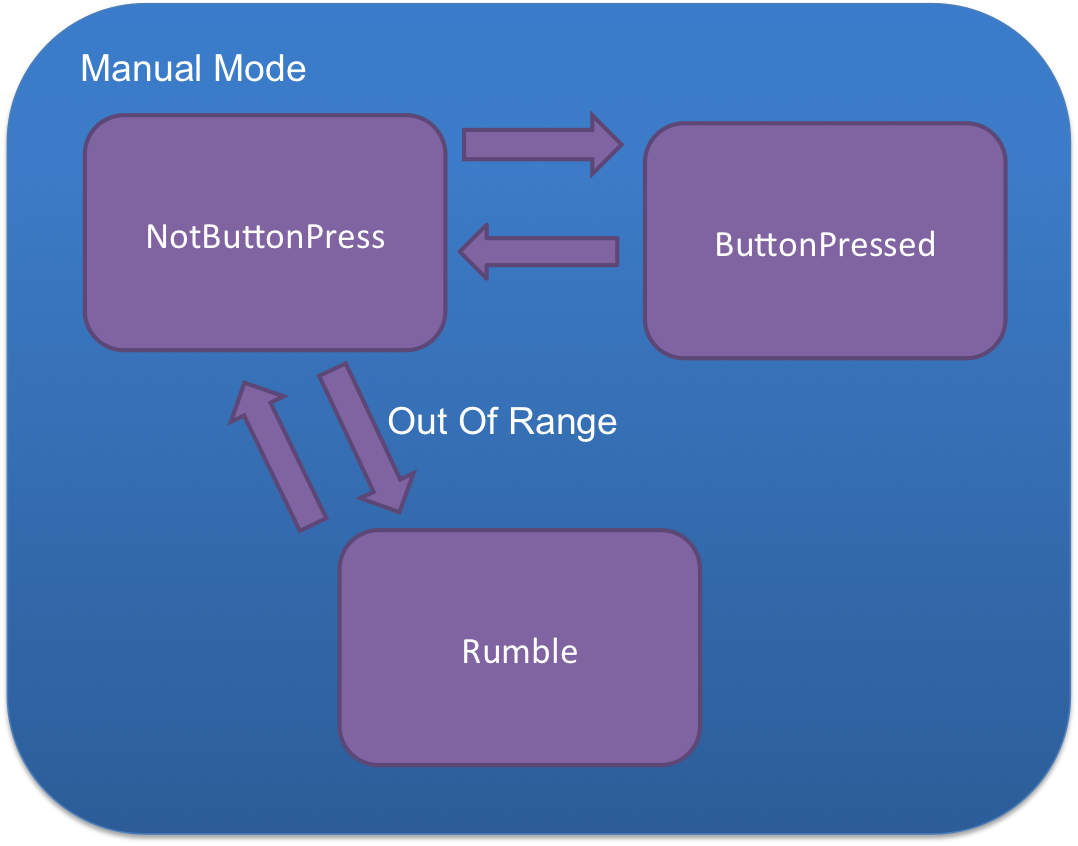
\includegraphics[width=1\linewidth]{../images/manual}
    \caption{Manual mode state machine model}
     \label{fig:manual_state}
    \end{center}
    \end{subfigure}
\end{center}

\caption{State Machines. The system is modeled as a hierarchical composition of state machines}
\label{fig:state_machines}
\end{figure}

\begin{figure}
\begin{center}
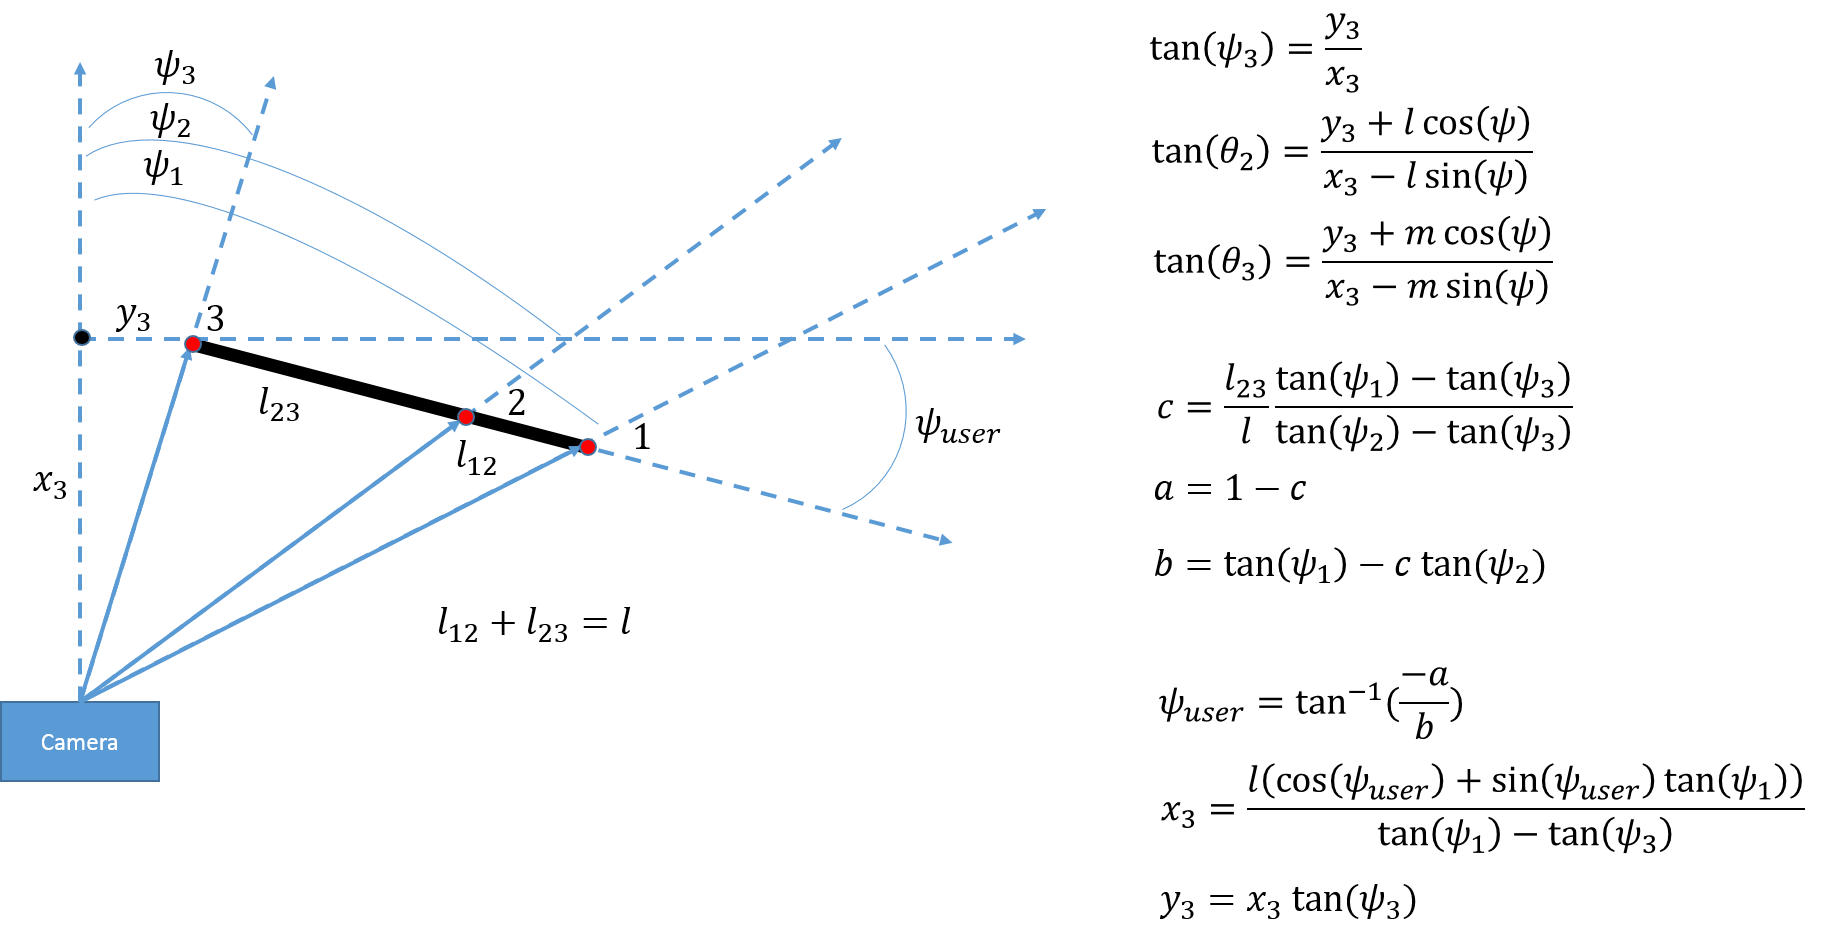
\includegraphics[width=\linewidth]{../images/geometry_and_equations_update}
\end{center}

\caption{State Reconstruction. By obtaining angular position measurements of three LEDs with known offsets, it is possible to fully reconstruct the state in a plane. Range data ($x_3$) obtained from one plane of measurement can be applied to aid state reconstruction in the other}
\label{fig:geometry}
\end{figure}

\section{Path Forward}
Originally, our project goal was to track the user's gaze, illuminating what the user was looking at on his or her desk. However, our algorithm proved too mathematically unstable for this, so we simplified the problem by having the light simply point at the user. Moving forward, we would like to explore more robust algorithms to solve the original problem. 

Moreover, we could explore other options of tracking the user's face. For instance, if we added an accelerometer to the hat, we could get further insight into what the user's head movements are, supplementing our existing algorithms with more data and reducing the effect of noise. Furthermore, we could investigate facial tracking or eyetracking, incorporating computer image or even video processing techniques to solve this problem. These other solutions could reinforce or replace our current tracking system, reducing the effect of input noise and possibly miniaturizing or entirely eliminating the headgear.

Another aspect that we could improve on is our physical design. Right now, the design is unpolished and unintuitive. The LED bars are mounted on cardboard taped to a hat, and our components are housed in a cardboard box. Moving forward, we would investigate the use of individual LED lights, so that the headgear is much more compact and usable. We would also strive to improve the user interface to SHaZam. Ideally, the user could start it up and enjoy its features with the push of a button. Ultimately, while there are many improvements yet to be made, we believe we have established a solid starting point with our work.


%\hfill mds
% 
%\hfill January 11, 2007
%
%\subsection{Subsection Heading Here}
%Subsection text here.
%
%
%\subsubsection{Subsubsection Heading Here}
%Subsubsection text here.


% An example of a floating figure using the graphicx package.
% Note that \label must occur AFTER (or within) \caption.
% For figures, \caption should occur after the \includegraphics.
% Note that IEEEtran v1.7 and later has special internal code that
% is designed to preserve the operation of \label within \caption
% even when the captionsoff option is in effect. However, because
% of issues like this, it may be the safest practice to put all your
% \label just after \caption rather than within \caption{}.
%
% Reminder: the "draftcls" or "draftclsnofoot", not "draft", class
% option should be used if it is desired that the figures are to be
% displayed while in draft mode.
%
%\begin{figure}[!t]
%\centering
%\includegraphics[width=2.5in]{myfigure}
% where an .eps filename suffix will be assumed under latex, 
% and a .pdf suffix will be assumed for pdflatex; or what has been declared
% via \DeclareGraphicsExtensions.
%\caption{Simulation Results}
%\label{fig_sim}
%\end{figure}

% Note that IEEE typically puts floats only at the top, even when this
% results in a large percentage of a column being occupied by floats.


% An example of a double column floating figure using two subfigures.
% (The subfig.sty package must be loaded for this to work.)
% The subfigure \label commands are set within each subfloat command, the
% \label for the overall figure must come after \caption.
% \hfil must be used as a separator to get equal spacing.
% The subfigure.sty package works much the same way, except \subfigure is
% used instead of \subfloat.
%
%\begin{figure*}[!t]
%\centerline{\subfloat[Case I]\includegraphics[width=2.5in]{subfigcase1}%
%\label{fig_first_case}}
%\hfil
%\subfloat[Case II]{\includegraphics[width=2.5in]{subfigcase2}%
%\label{fig_second_case}}}
%\caption{Simulation results}
%\label{fig_sim}
%\end{figure*}
%
% Note that often IEEE papers with subfigures do not employ subfigure
% captions (using the optional argument to \subfloat), but instead will
% reference/describe all of them (a), (b), etc., within the main caption.


% An example of a floating table. Note that, for IEEE style tables, the 
% \caption command should come BEFORE the table. Table text will default to
% \footnotesize as IEEE normally uses this smaller font for tables.
% The \label must come after \caption as always.
%
%\begin{table}[!t]
%% increase table row spacing, adjust to taste
%\renewcommand{\arraystretch}{1.3}
% if using array.sty, it might be a good idea to tweak the value of
% \extrarowheight as needed to properly center the text within the cells
%\caption{An Example of a Table}
%\label{table_example}
%\centering
%% Some packages, such as MDW tools, offer better commands for making tables
%% than the plain LaTeX2e tabular which is used here.
%\begin{tabular}{|c||c|}
%\hline
%One & Two\\
%\hline
%Three & Four\\
%\hline
%\end{tabular}
%\end{table}


% Note that IEEE does not put floats in the very first column - or typically
% anywhere on the first page for that matter. Also, in-text middle ("here")
% positioning is not used. Most IEEE journals/conferences use top floats
% exclusively. Note that, LaTeX2e, unlike IEEE journals/conferences, places
% footnotes above bottom floats. This can be corrected via the \fnbelowfloat
% command of the stfloats package.



%\section{Conclusion}
%The conclusion goes here.
%
%
%
%
%% conference papers do not normally have an appendix
%
%
%% use section* for acknowledgement
%\section*{Acknowledgment}
%
%
%The authors would like to thank...





% trigger a \newpage just before the given reference
% number - used to balance the columns on the last page
% adjust value as needed - may need to be readjusted if
% the document is modified later
%\IEEEtriggeratref{8}
% The "triggered" command can be changed if desired:
%\IEEEtriggercmd{\enlargethispage{-5in}}

% references section

% can use a bibliography generated by BibTeX as a .bbl file
% BibTeX documentation can be easily obtained at:
% http://www.ctan.org/tex-archive/biblio/bibtex/contrib/doc/
% The IEEEtran BibTeX style support page is at:
% http://www.michaelshell.org/tex/ieeetran/bibtex/
%\bibliographystyle{IEEEtran}
% argument is your BibTeX string definitions and bibliography database(s)
%\bibliography{IEEEabrv,../bib/paper}
%
% <OR> manually copy in the resultant .bbl file
% set second argument of \begin to the number of references
% (used to reserve space for the reference number labels box)
%\begin{thebibliography}{1}
%
%\bibitem{IEEEhowto:kopka}
%H.~Kopka and P.~W. Daly, \emph{A Guide to \LaTeX}, 3rd~ed.\hskip 1em plus
%  0.5em minus 0.4em\relax Harlow, England: Addison-Wesley, 1999.
%
%\end{thebibliography}




% that's all folks
\end{document}


